\chapter{Background}
\label{Chapt2}
This chapter will cover the basic background of rowing, the sports science which guides rowing training, and how an athletes body responds to training stimulus. Next, a review of performance modelling will explore the development of human performance modelling since the introduction of the basic Bannister model in 1975 \autocite{Bannister1976}. The section will outline how training load and performance can be quantified, and explain the way these approximations are used in various performance models to date.

\section{A brief introduction to rowing}
Rowing is an Olympic sport, raced across a 2,000 metre course, typically lasting six to seven minutes. It is classed as a power-endurance sport, this means training is focused on building aerobic, anerobic, and power while also developing rowing technique \autocite{Mäestu2005}. Most time is spent building endurance, next most time is spent building anerobic capacity, finally building strength and power through Strength and Condition sessions \autocite{Seiler2006}. The importance of power is more significant in rowing than in cycling given the relatively short duration of exertions, with longer distance racing typically only covering five to seven kilometers, or fifteen to twenty-five minutes. Road cycling, for example, tends to last for a longer period of time, where the shortest races might last two hours. There are many different approaches to how training is conducted and which energy systems are targeted. This section will discuss the basic training principles which guide training, the way athletes respond to different kinds of training loads, and how performance is evaulated in rowing. 

\subsection{Training Principles} \label{sub:training_principles}
Generally when a coach builds a training plan they have a few factors they can work with: volume, the amount of mileage or total time spent training, sessions intensity, how hard the given session is meant to be, and finally the frequency, or the time spent in different intensity zones. There are various ways to measure intensity, including heart rate, blood lactate concentration, velocity at maximal oxygen uptake (VO2 max), and rate of perceived exertion (RPE) \autocite{Rosenblat2019}. Rowers tend to use heart rate zones or blood lactate concentration depending on access to the equipment to test blood lacate. Typically when a rower uses calculated aerobic zones each zone will be a percentage of \maxHR. Following this approach, zones are defined as follows:
\begin{description}
  \item[Z1] "Very Light" intensity, 50\% - 60\% of \maxHR
  \item[Z2] "Light" intensity, 60\%-70\% of \maxHR
  \item[Z3] "Moderate" intensity, 70\%-80\% of \maxHR
  \item[Z4] "Hard" intensity, 80\%-90\% of \maxHR
  \item[Z5] "Maximum" intesity, 90\%-100\% of \maxHR
\end{description}
The exact definition of these zones varies in the literature, as does the method to calculate \maxHR without a specific test. However, most high level athletes will have completed some kind of stress test to determine their \maxHR in order to train more effectively on their prescribed zones.
A rower who uses lactate based training zones might use the following zones:
\begin{description}
  \item[T1]  basic oxygen utilization training (UT2) [lactate~=~0-2 mmol/L]
  \item[T2]  oxygen utilization training (UT1) [lactate~=~2-3.5 mmol/L]
  \item[T3]  anaerobic threshold training (AT) [lactate~=~3.5-4.5 mmol/L]
  \item[T4]  oxygen transport training (TR) [lactate~=~4.5-6 mmol/L]
  \item[T5]  anaerobic capacity training (AN) [lactate $\geq$ 6 mmol/L] \autocite{Das2022}
\end{description}
Depending on how rigorous the testing protocol was, Heart Rate zones may be calculated for each zone, these may vary from the aerobic zones calculated from \maxHR. 

The most basic zone approximation approach uses three zones based around certain physiological thresholds, like, lacate thresholds ($\textnormal{LT}_\text{1}$ and $\textnormal{LT}_\text{2}$) and ventilatory thresholds. Cyclists may use critical power to determine these three basic zones, although this practice has not become popular in rowing training. The zones become simply, low-intensity, moderate-intensity, and high-intensity. 

There are a few different approaches for distributing intensity for endurance training. The three main methods are: polarised training, sweet spot or threshold training, and pyramidal training. This guides the final factor a coach considers when building a general training plan, frequency. For the purposes of comparing polarized training (POL), threshold training (THR), and pyramidal training (PYR), the more basic three zones of intensity will be used. The breakdown per zone for each training method is as follows:
\begin{description}
  \item[Polarised Training] Far more time spent in the low-intensity zone \autocite{Seiler2004}.

  \begin{description}
    \item[Low-Intensity] 75\%-85\% of total training volume
    \item[Medium-Intensity] 5\%-10\% of total training volume
    \item[High-Intensity] 5\%-10\% of total training volume  
  \end{description} 
  \item[Threshold Training] More time spent in the medium-intensity zone \autocite{Seiler2004}.

  \begin{description}
    \item[Low-Intensity] 45\%-55\% of total training volume
    \item[Medium-Intensity] 35\%-55\% of total training volume
    \item[High-Intensity] 15\%-20\% of total training volume  
  \end{description}
  \item[Pyramidal Training] Most time spent in low-intensity zone with progressively less time spent in higher zones \autocite{Selles2019}.

  \begin{description}
    \item[Low-Intensity] 75\%-85\% of total training volume
    \item[Medium-Intensity] 15\%-20\% of total training volume
    \item[High-Intensity] 5\%-10\% of total training volume  
  \end{description}
\end{description}

This report will not compare the effectiveness of different training distributions. Different distributions tend to be used by different sports, or depending on which energy system is being targeted. The use of polarized training is most common in rowing \autocite{Rosenblat2019}, although other training approaches have been used, especially around competition time.


\subsection{Energy Systems}
\label{sub:energy_systems}
In the human body there are two major types of skeletal muscle fibres, fast twitch, and slow twitch. Slow twitch muscles are used for longer, slower contractions where relative strength is low. Conversely, fast twitch muscles are shorter, faster contractions where strength is relatively higher. These types of fibres store energy differently and respond to training differently. Slow twitch muscles can be adapted to longer, lower effort, sessions and become resistant to fatigue, while fast twitch muscles fatigue easily, due to their lower glycogen capacity. Slow twitch muscle fibres have a low anaerobic capacity, while fast twitch muscle fibres have high anerobic capacities. These two kinds of fibres draw on two different energy systems: anaerobic and aerobic systems. These systems provide muscles with Adenosine Triphosphate (ATP) which is used by the mitochondria in the muscle fibre cells to produce energy, allowing the muscles to contract \cite{Göktepe2007}. 

The anaerobic system is used to provide energy to muscles to produce power without the use of oxygen. The anaerobic system typically provides energy for shorter periods of time. An immediate energy system can provide energy for 1-2 seconds of maximal work, this is typically used for resistance based strength training. More commonly in rowers, the short term energy system is used to provide energy to muscle fibres under significant strain. However, each time the energy system produces (ATP), lactate is also produced. This system is limited by an athletes ability to flush lactate from muscles. If the muscles are unable to flush the lactate quickly enough, the muscles will fatigue until exercise needs to stop. 

The aerobic, or long term energy, system is the slowest at providing energy to muscles. This system uses sugars, fats and oxygen to produce ATP. This system only works when large amounts of oxygen are available, which for rowers is typically during lower intensity sessions. Longer "steady state" sessions rely on the aerobic to provide energy to muscles, with these sessions also being used to build the aerobic system. By spending time in the appropriate training zones the aerobic system builds efficiency by creating new capillaries to support the slow twich fibres.

Rowers develop both their anaerobic and aerobic systems. Much of the winter season (typically September-March) is spent building the aerobic system, this is due to the longer length of any races done during this period, and to build a larger base on which to build a strong anerobic system. As the sprint racing season begins, or shortly before, more anerobic sessions will be introduced to build the system. Rowers will build their lactate tolerance, and spend more time at just-below-maximal efforts to prepare for the shorter race format.

% \subsection{Physiological Response to Training}
% Different people respond to training differently, for example, two people may be taking up a similar volume of oxygen (even $\textnormal{VO}_2$ utilization), but their muscles may be responding differently, producing different performances, or being able to sustain that load for different length of time. Differences in lactate threshold (LT), for example, can model the physiological state of an athlete during these efforts \autocite{Baldwin2000}. The goal for each training session is to, as efficiently as possible, become "fitter", in order to perform better. \textcite{Seiler2011} (2011) explored the effect of the use of different training intensities and durations on trained cyclists. 4x8min interval sessions yielded the most "\textit{pain for the gain}". Given that 


\subsection{Performance}
There are two primary ways to measure a performance in rowing. First, on the rowing machine, a 2,000 meter, 6,000 meter, or 30 minute at stroke rate 20 (30 r20) test is normally used, depending on when during the season the test is done. This can be used to determine a rowers fitness and can be used to track progress for an athlete. These sessions are typically maximum effort sessions with some degree of taper (typically 4-7 days maximum) to illicit a peak performance. On the water, times can also be used to judge an entire crew, with external factors like wind direction and intensity, current flow, and temprature considered. Some boats and squads may use on the water telemetry to quantify the impact and power output of each rower. On the water performances may not always be peak efforts depending on a squads seasonal focus or an event's progression (eg. a maximal effort will rarely make an appearance in the heat stage of a heat-semi-final progression). Ergometer scores tend to be the pureset way of quantifying rowers performance, however a combination of approaches can be used to quantify on the water performance.

\subsection{Summary}
Rowing training is quite time consuming for athletes. Many rowers will learn much of what has been discussed in this section to make better decisions themselves, or understand why training is done in a given way. The focus for a majority of the training cycle is to build a strong aerobic base in order to allow for higher "peak", ideally coinciding with the peak event for a season of training. For international athletes this will be a yearly cycle targetting World Championships, which is part of a four-yearly cycle targetting the Olympics. For national level athletes, national championships are typically the target, with Henley Royal Regatta featuring as a seasons target. Coaches will normally take into account season targets and rower proficiency and base fitness when generating training plans. The target of this project is to make it easier for coaches and more accessible for more independent athletes. 

\section{A Review of Performance Modelling}
The first wide spread approach to modelling performance was developed by \textcite{Bannister1976} with the Banister Fitness - Fatigue model, and further refined by \textcite{Morton1990} when defining training impulse to determine fitness and fatigue. The use of machine learning, specifically artifical neural networks has since been introduced in approaches to model performance. In preparation for the 2000 Olympics in Sydney \textcite{Edelmannnusser2002} successfully predicted olympic performances within an error of 0.05 seconds across a total time of 2:12.64 (min:sec) for the 200m backstroke event. \textcite{Edelmannnusser2002} specifically consider the limitation of using a linear model, such as the model proposed by \textcite{Bannister1976}, on training adaptation and performance; adaptation to training is inherently a complex non-linear process. 

This chapter will review basic approaches to systems modelling, exploring metrics which are commonly used to guide models and some non-linear systems models which have been explored.

\subsection{Quantifying Training Load (Fatigue)}
\subsubsection{Rate of Perceived Exertion (RPE)} \label{subsub:rpe}
Rate of perceived exertion (RPE) is a scale, originally introduced by Gunnar Borg, to measure an athletes effort. The original scale ranged from 6-20, where 6 would be no exertion at all, and 20 is maximal effort. This scale ranges from 6-20 to correspond more easily with heart rate, as the scale is used beyond just athletic settings. Therefore another scale, ranging from 0-10, was developed by Borg as well for use with "extreme intensity of activity", this is the scale normally used in athletic studies. The second scale is called a Category-Ratio (CR) scale where the reference anchor is RPE CR10 of 10, meaning maximal effort/pain. Session RPE (sRPE), using CR10, can be used, in conjunction with duration to determine session load \cite{Williams2017}.

\begin{figure}[!h]
  \begin{minipage}[c]{0.4\linewidth}
      \centering
      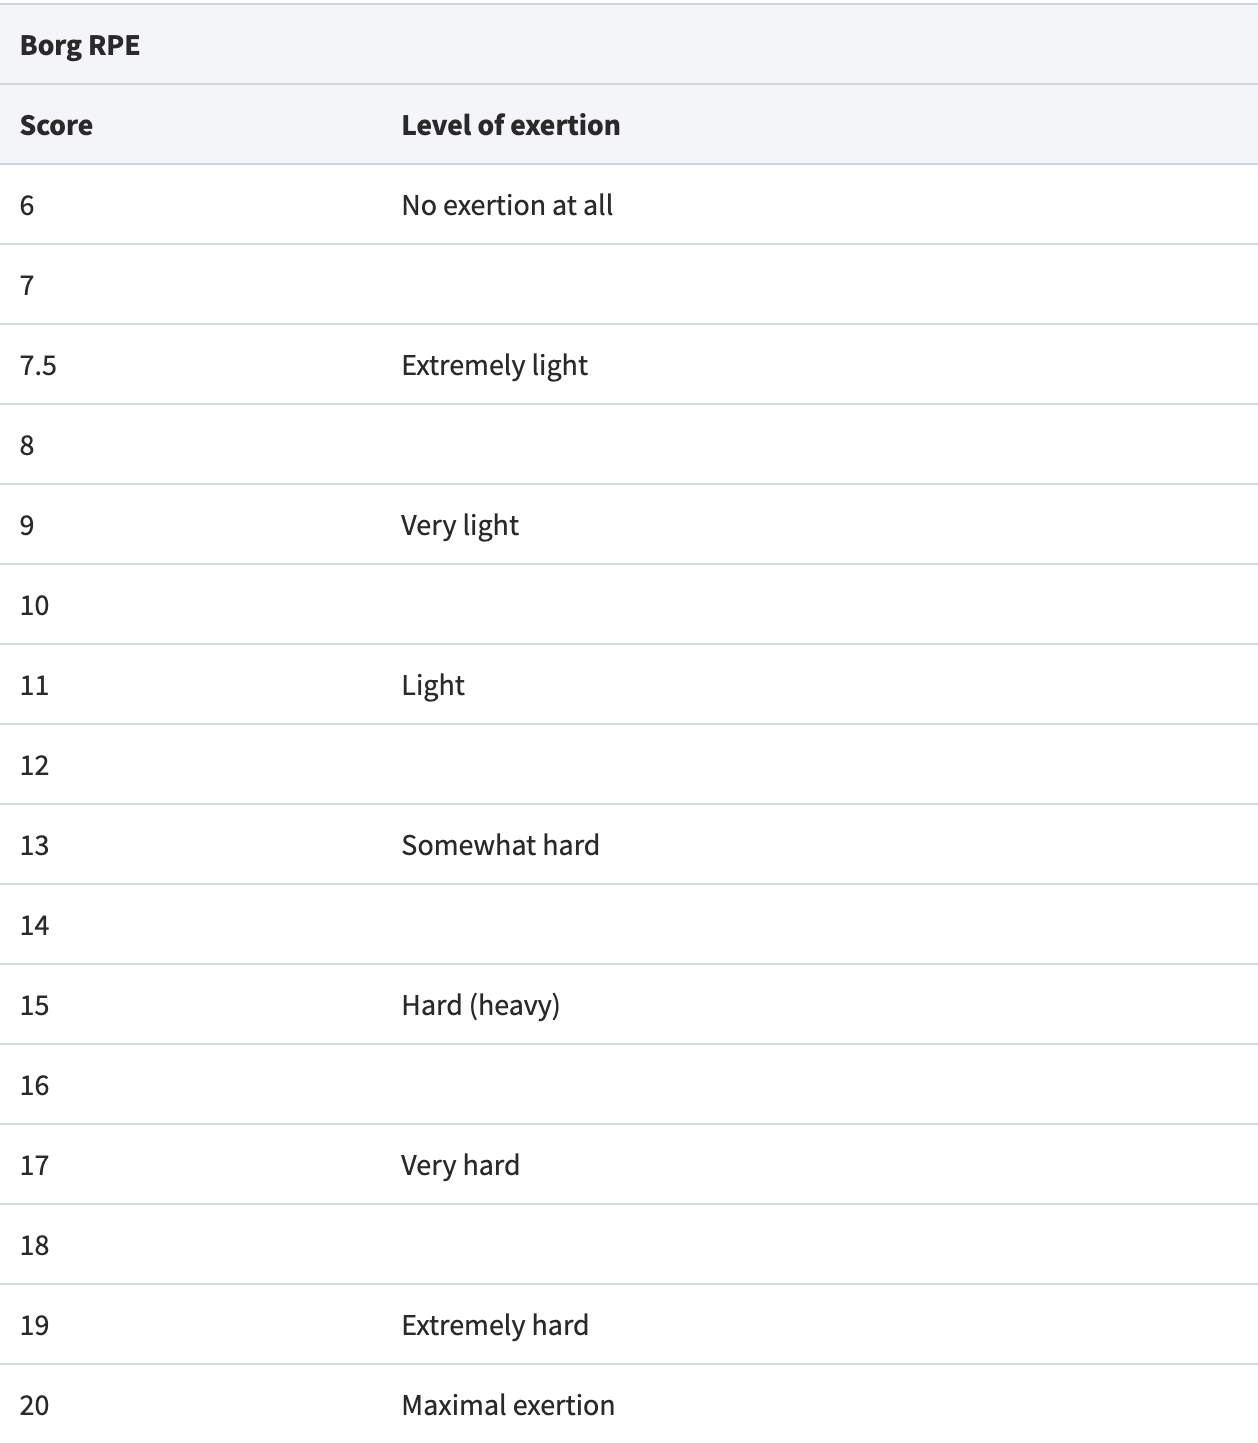
\includegraphics[width=\linewidth]{figures/borg20.png}
      \captionsetup{justification=centering}
      \caption[Borg 20]{The original Borg 6-20 RPE Scale \cite{Williams2017}} \label{fig:borg20}
  \end{minipage}\hfill
  \begin{minipage}[c]{0.4\linewidth}
      \centering
      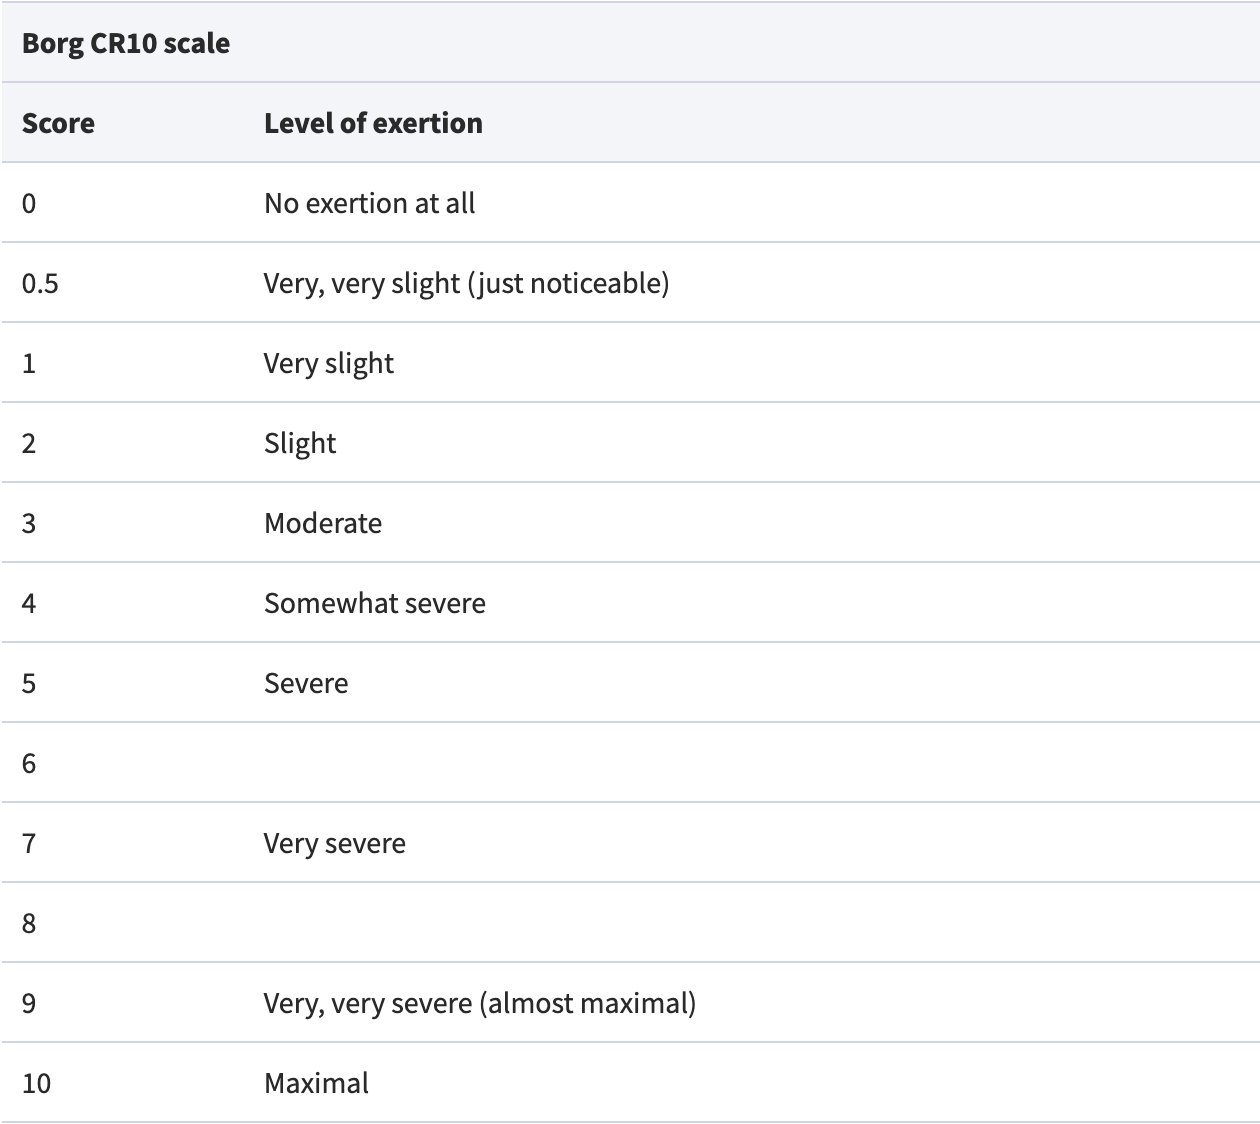
\includegraphics[width=\linewidth]{figures/borgc10.png}
      \captionsetup{justification=centering}
      \caption[Borg CR10]{The Borg Category-Ratio 10 RPE Scale \cite{Williams2017}}\label{fig:borgcr10}
  \end{minipage}
  \caption*{The two Borg RPE scales}
\end{figure}

\subsubsection{Training Impulse (TRIMP)}
Training Impulse (TRIMP) is a method to calculate training load and is defined as  $\textnormal{TRIMP} = \textnormal{Training Volume} \times \textnormal{Training Intensity}$ \autocite{TRIMPmethod}. There are many methods to calculate TRIMP, using different metrics to calculate training volume and training intensity. For the purposes of this project volume will simply be minutes, and intensity will be average heart rate (bpm), as the simplest TRIMP method outlined. Other modifications of may apply a weighting against a heart rate metric to normalise longer sessions completed at a lower heart rate -- considering the noted difference in heart rate responses to training in male and female athletes \autocite{Morton1990}, alternatively load can be calculated by using the product of RPE and duration (ie. $\textnormal{RPE} \times \textnormal{Duration (minutes)}$) .

\subsubsection{Acute Chronic Workload Ratio (ACWR)}
Acute Chronic Workload Ratio (ACWR) can be used to monitor load in an athlete. It compares training load accumulated, in arbitrary units (AU), over the last seven days (acute workload) to the training load accumulated over the last twenty-eight days (chronic workload). The exact calculations used to determine acute and chronic workload depends on what type of ACWR model is selected. Additionally, the exact time periods considered for acute and chronic load can change depending on the application \cite{White2023}. Typically ACWR is used for injury management in team sports, but some articles have found it may not be effective for preventing injury as it is inaccurate way of approximating load \cite{Impellizzeri2020}. Regardless of it's effectiveness in reducing injury, ACWR charts are easy to produce and provide easy feedback to rowers to see how their training load can change week-to-week.

\subsection{Impulse-Response Models} 
\subsubsection{Banister Fitness-Fatigue Model}

\subsubsection{Limitations to the Impulse-Response Model}

\subsection{Alternative Models}
\subsubsection{Performance Potential (PerPot)}
\subsubsection{Artificial Neural Network (ANN) approaches}
